\documentclass[./main.tex]{subfiles}
% \usepackage{pgfplots}

\begin{document}
    \subsubsection*{問4}
    \addcontentsline{toc}{subsubsection}{問4}
    \markboth{2024年 統計数理 問4}{2024年 統計数理 問4}


    \begin{enumerate}

        % TikZ 通りますよ~
        \begin{figure}[h]
            \centering
            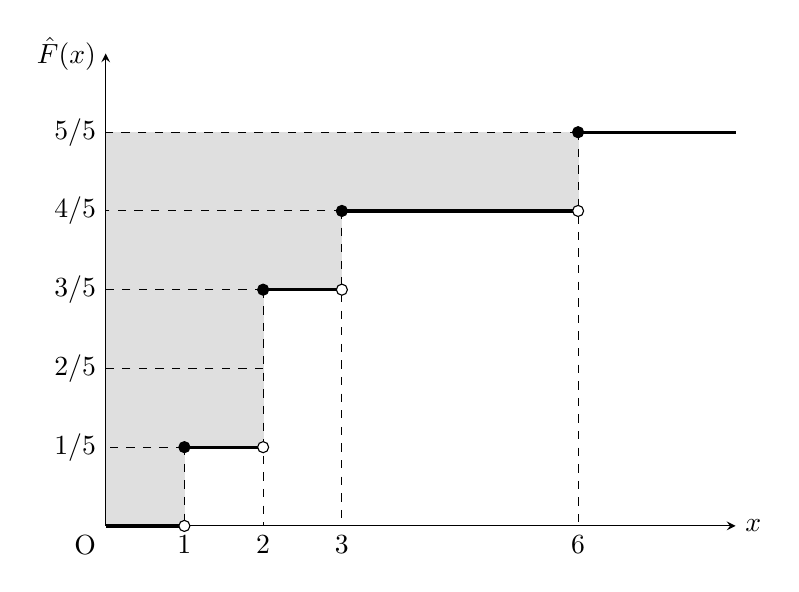
\begin{tikzpicture}[yscale=5]
                % [2] の面積
                \filldraw[lightgray!50!white] (0, 0)--(1, 0)--(1, 0.2)-- (2, 0.2)
                    --(2, 0.6)--(3, 0.6)--(3,0.8)--(6, 0.8)--(6, 1.0)--(0, 1.0) --cycle;


                % 原点
                \node [below left] (0, 0) {O};
                % x 軸
                \draw[-stealth] (0, 0)--(8.0, 0) node[right] {$x$};
                % y 軸
                \draw[-stealth] (0, 0)--(0, 1.2) node[left] {$\hat{F}(x)$};

                % 線
                \draw[very thick] (0, 0)--(1.0, 0);
                \draw[very thick] (1, 0.2)--(2, 0.2);
                \draw[very thick] (2, 0.6)--(3, 0.6);
                \draw[very thick] (3, 0.8)--(6, 0.8);
                \draw[very thick] (6, 1.0)--(8, 1.0);

                % 横点線
                \foreach \x / \y in {1/{1/5}, 2/{2/5}, 2/{3/5}, 3/{4/5}, 6/{5/5}} {
                    \draw[dashed] (\x, \y) -- (0, \y) node [left] {$\y$};
                }
                % \draw[dashed] (1.0, 0.2)--(0, 0.2) node [left] {$1/5$};
                % \draw[dashed] (2.0, 0.6)--(0, 0.6) node [left] {$3/5$};
                % \draw[dashed] (3.0, 0.8)--(0, 0.8) node [left] {$4/5$};
                % \draw[dashed] (6.0, 1.0)--(0, 1.0) node [left] {$5/5$};

                % 縦点線
                \draw[dashed] (1, 0.2)--(1, 0) node[below] {$1$};
                \draw[dashed] (2, 0.6)--(2, 0) node[below] {$2$};
                \draw[dashed] (3, 0.8)--(3, 0) node[below] {$3$};
                \draw[dashed] (6, 1.0)--(6, 0) node[below] {$6$};

                % 点
                % y 方向定に伸びてしまうので一次的に yscale を 0.2 倍します。
                % その影響で、y 座標も 5 倍で指定しないといけません。
                \begin{scope}[transform shape, yscale=0.2]
                    % 黒丸
                    \foreach \Point in {(1, 1), (2, 3), (3, 4), (6, 5)} {
                        \draw [fill=black] \Point circle (2pt);
                    }
                    % 白丸
                    \foreach \Point in {(1, 0), (2, 1), (3, 3), (6, 4)} {
                        \draw [fill=white] \Point circle (2pt);
                    }

                \end{scope}

            \end{tikzpicture}
            \caption{経験分布関数}
        \end{figure}

        % (1)
        \item 図のようになる。

        %%%%%%%%%%%%%%%%%%%%%%%%%%%%%%%%%%%%%%%%%%%%%%%%%%%
        % [2]
        %%%%%%%%%%%%%%%%%%%%%%%%%%%%%%%%%%%%%%%%%%%%%%%%%%%
        \item 標本平均は $\dfrac{1}{5} (1 +2 + 2 + 3 + 6)$ と書け、図の色を塗った部分の面積がそれに対応する。\\


        %%%%%%%%%%%%%%%%%%%%%%%%%%%%%%%%%%%%%%%%%%%%%%%%%%%
        % [3]
        %%%%%%%%%%%%%%%%%%%%%%%%%%%%%%%%%%%%%%%%%%%%%%%%%%%
        \item 右辺から変形する。$1 -F (x) = P(X > x)$ であるから

            \begin{minipage}[l]{0.6\textwidth}
                \begin{equation*}
                    \int_0^\infty \left\{ 1 - F(x) \right\} \, dx
                        = \int_0^\infty \left\{ \int_x^\infty f(y) \, dy \right\} \, dx
                \end{equation*}
                ここで 積分の順序を入れ替える。
                積分領域は図の青矢印から赤矢印のようになる事に注意すると、
                \begin{equation*}
                    = \int_0^\infty \left\{ \int_0^y f(y) \, dx \right\} \, dy
                        = \int_0^\infty y f(y) \, dy
                        = E[X].
                \end{equation*}
            
            \end{minipage}
            \hfill
            %%%%%%%%%%%%%%%%%%%%%%%%%%%%%%%
            % ここ改行したらアカン
            %%%%%%%%%%%%%%%%%%%%%%%%%%%%%%%
            \begin{minipage}[c]{0.3\textwidth}
                \centering
                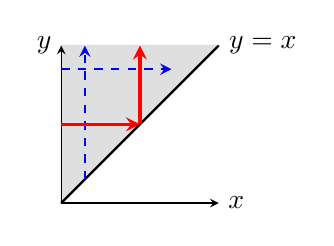
\begin{tikzpicture}
                    % 領域
                    \filldraw[lightgray!50!white] (0, 0)--(2, 2)--(0, 2)--cycle;

                    % 軸とグラフ
                    \draw[-stealth] (0, 0)--(2, 0) node [right] {$x$};
                    \draw[-stealth] (0, 0)--(0, 2) node [left] {$y$};
                    \draw[thick] (0, 0)--(2, 2) node [right] {$y=x$};

                    % 矢印
                    \draw[-stealth, thick, blue, dashed] (0.3, 0.3)--(0.3, 2.0);
                    \draw[-stealth, thick, blue, dashed] (0, 1.7)--(1.4, 1.7);

                    \draw[-stealth, very thick, red] (0, 1.0)--(1.0, 1.0);
                    \draw[-stealth, very thick, red] (1.0, 1.0)--(1.0, 2.0);

                \end{tikzpicture}
            \end{minipage}\\

        \item  $x\geq 0$ として
        \begin{align*}
            f(x)
            &= \int_0^\infty ( \lambda e^{-\lambda x} ) \cdot 
                \left\{ \frac{\beta^\alpha}{\Gamma (\alpha)} \lambda^{\alpha - 1} e^{\beta \lambda} \right\} \, d\lambda
                = \frac{\beta^\alpha}{\Gamma (\alpha)} \int_0^\infty \lambda^{(\alpha + 1) - 1} e^{-(x + \beta) \lambda} \, d\lambda\\
            &= \frac{\beta^\alpha}{\Gamma (\alpha)} \cdot \frac{ \Gamma (\alpha + 1)}{(x + \beta)^{\alpha + 1}} 
                = \frac{\alpha \beta^\alpha}{(x + \beta)^{\alpha + 1}}.
        \end{align*}

        % 5
        \item 
        \begin{align*}
            E[X + \beta]
                &= \int_0^\infty (x + \beta) \cdot \frac{\alpha \beta^\alpha}{(x + \beta)^{\alpha + 1}}
                = \alpha \beta^\alpha \int_0^\infty \frac{1}{(x + \beta)^\alpha} \, dx
        \end{align*}
        $\alpha = 1$ の時、積分は $\displaystyle \left[ \log (x + \beta) \right]_0^\infty$ となって発散する。
        $\alpha \neq 1$ の時は $\displaystyle \frac{1}{1 - \alpha} \left[ \frac{1}{(x + \beta)^{\alpha-1}}  \right]_0^\infty$ となり、
        $(0 < ) \, \alpha < 1$ で発散する。
        すなわち、収束条件は $\alpha > 1$ であり、このとき
        \begin{equation*}
            E[X] 
                = -\beta + \alpha\beta^\alpha \cdot \frac{1}{1-\alpha} \cdot \frac{-1}{\beta^{\alpha - 1}}
                = \frac{\beta}{\alpha - 1}.
        \end{equation*}



    \end{enumerate}

    % ~~~~~~~~~~~~~~~~~~~~~~~~~~~~~~~~~~~~~~~~~~~~~~~~~~~~~~~~~~~~~
    % ~~~~~~~~~~~~~~~~~~~~~~~~~~~~~~~~~~~~~~~~~~~~~~~~~~~~~~~~~~~~~
    \subsubsection*{コメント}
    経験分布関数を知らないと死ぬ問題である。
    逆に、知っていたら比較的手を付けやすい問題であるとも言える。
    統計検定ではこういった、知ってるとすぐだが知らないとどうにもならない問題が割と多いのでなかなか難しいところである。

    小問についても [3] までと [4] 以降でだいぶ毛色が違うセットになっており、正直なところ出題意図がよくわからない。
    [5] を [3] の結果を使って計算できないこともないが、ふつうに $E[X + \beta]$ を計算した方が早いという本末転倒ぶりである。
    そのため、経験分布関数なんて知らねぇ!って方でも [4] と [5]、場合によっては比較的有名な問題である [3] にも手を付けられたのではなかろうか。


    \begin{enumerate}
        % 1
        \item 経験分布関数 (eCDF; expirical cumulative distribution function) は、標本 $x_1, x_2, \dots, x_n$ を小さい順にカウントしていく関数で、
        次のように定義されます。
        \begin{equation}
            \hat{F}_n (x)
                = \frac{1}{n} \sum_{i=1}^n 1_{ \{ x_i \leq x \} }
        \end{equation}
        得られた標本の中に $x$ 以下のものがいくつあるか数え、最後に標本の大きさ $n$ で割ったものが $\hat{F}_n (x)$ という事です。
        これにより、$x$ が標本の最小未満だと $0$、最大以上だと $1$ になり、累積分布関数 (CDF) っぽいものになっていることが分かります。
        実際、eCDF は大数の強法則によって CDF に概収束することが示されるので、未知の確率分布を推定する時に $\hat{F}_n (x)$ が使用できるらしいです。

        グラフを描いてみると、CDF 同様に右連続左極限 (右から左に攻めると黒丸、左から右に攻めると白丸) になっていることも分かります。


        % 2
        \item \relax [3] への布石となります。
        
        % 3
        \item \relax [2] で色を塗った部分が $\displaystyle \int_0^\infty \left\{ 1 - \hat{F}_5 (x) \right\} \, dx$ で、
        その値も $\displaystyle 1 \cdot \frac{1}{5} + 2 \cdot \frac{2}{5} + 3 \cdot \frac{1}{5} + 6 \cdot \frac{1}{5}$ と
        期待値の式っぽく書けるので、与えられた式も何だか正しそうに見えてきます。
        そしてこの期待値 (?) の式、$x$ の値を $\hat{F}$ 方向に積分しているように見えませんか?
        おそらくそういう問題だと思います。

        こういう "$\hat{F}$ 方向の積分" のことをスティルチェス積分と言いますが、この問題ではスティルチェス積分を仄めかしつつ、
        積分の順序交換でこれを計算させようとしています。
        順序交換に伴って積分範囲も変わってきますが、これは慣れないとけっこう難しいし、言語化して説明するのも難しいので慣れるしかないと思います。

        なお、今回は非負確率変数 $X$ とその実現値についての話でしたが、負の値も取りうる場合には次のような式になります。
        \begin{equation}
            E[X] 
                = - \int_{-\infty}^0 F(x) \,dx
                    + \int_0^\infty \left\{ 1 - F(x) \right\} \, dx
        \end{equation}


        % 4
        \item と思っていたら、唐突な混合分布の問題です。

        ここでは、ガンマ関数の定義が
        \begin{equation}
            \Gamma (\alpha) 
                = \int_0^\infty x^{\alpha - 1} e^{-x} \, dx
                \qquad (\alpha > 0)
        \end{equation}
        で与えられることを使っています。
        分母に $(x + \beta)^{\alpha + 1}$ が現れているところは、気持ちとしては下のような計算をしています。
        $c > 0$ を正の定数として
        \begin{equation*}
            \int_0^\infty x^{\alpha - 1} e^{-cx} \, dx
                = \frac{1}{c^\alpha} \int_0^\infty (cx)^{\alpha - 1} e^{-cx} \, d(cx)
                = \frac{1}{c^\alpha} \Gamma (\alpha)
        \end{equation*}
        $cx$ の関数とみて、ガンマ関数の定義の形を無理やり作っているんですね。
        % $x^{\alpha-1}$ のところで $\alpha - 1$ 個、$dx$ のところで $1$ 個余分に掛けることになるので、
        このように考えると置換積分をする旨を文章で書かなくて良くなるので早くなります。
        よく出る形なので慣れておくと良いでしょう。
        
        実際、それなりに応用力もあって、例えばガウス積分 $\displaystyle \int_{-\infty}^\infty e^{-x^2} \, dx = \sqrt{\pi}$ の $e$ の肩が定数倍されたものも
        \begin{equation*}
            \int_{-\infty}^\infty e^{-cx^2} \, dx
                = \frac{1}{\sqrt{c}} \int_{-\infty}^\infty e^{-(\sqrt{c} x )^2} \, d(\sqrt{c}x)
                = \sqrt{ \frac{\pi}{c}}
        \end{equation*}
        といったように計算できます。


        \item そして出てきたのはパレート分布だったのでした。

        
    \end{enumerate}


\end{document}